\documentclass{jpsj2}
% 2002/12/16
%\usepackage[mtbold]{mathtime}

\def\runtitle{Instructions for the Preparation of Manuscript}
\def\runauthor{Online-Journal Subcommittee}

\title{%
Instructions for the Preparation of a Manuscript for \\
the \textit{Journal of the Physical Society of Japan}
}

\author{%
Online-Journal Subcommittee of JPSJ\thanks{E-mail address: jpsj-online@jpsj.or.jp}
}

\inst{%
The Physical Society of Japan, Tokyo 105-0011
}

\recdate{\today}

\abst{%
This document explains how to prepare manuscripts for the \textit{Journal of 
the Physical Society of Japan} using the \LaTeXe{} class file ``jpsj2.cls''.
}

\kword{%
\LaTeXe, amsmath.sty, graphicx.sty, EPS, PDF
}

\begin{document}
\maketitle

\section{Introduction}

\LaTeXe{} has recently replaced the old version of \LaTeX{} 2.09.  In order to use more convenient macros provided as the standard \LaTeXe{} distribution, we have prepared a \LaTeXe{} class file, \texttt{jpsj2.cls}, for the \textit{Journal of the Physical Society of Japan} (JPSJ), which is based on the former \LaTeX{} style file, \texttt{jpsj.sty}.

The basic usage of this class file is the same as that with \texttt{jpsj.sty}.  Please note that we \emph{continue} to accept \LaTeX{} 2.09-based manuscripts as well.

For basic usage of \LaTeXe{}, the standard reference will help you.~\cite{blue}

\section{Changes}

\subsection{Discarded}

Since \texttt{jpsj2.cls} is designed only for submission to JPSJ, we have discarded (1) \texttt{full} environment, (2) \texttt{short} option and (3) \texttt{preprint} option.

\subsection{Font selection}

A major difference between \LaTeXe{} and \LaTeX 2.09 is the mechanism of font selection (see Table~\ref{t1}).  We recommend that authors use the new commands although \texttt{jpsj2.cls} is compatible with the old commands. 

\begin{table}[t]
\caption{New and old commands for font selection.}
\label{t1}
\begin{center}
\begin{tabular}{@{\hspace{\tabcolsep}\extracolsep{\fill}}cc|c} \hline
New & Old & Output \\ \hline
\verb|\textbf{boldface}| & \verb|{\bf boldface}| & \textbf{boldface} \\
\verb|\textit{italic}| & \verb|{\it italic}| & \textit{italic} \\
\verb|\textsf{sans serif}| & \verb|{\sf sans serif}| & \textsf{sans serif} \\
\verb|\textsc{Small Capital}| & \verb|{\sc Small Cap}| & \textsc{Small Cap} \\
\verb|\emph{emphasis}| & \verb|{\em emphasis}| & \emph{emphasis} \\
\hline
\verb|\mathcal{CALLIGRAPHY}| & \verb|{\cal CALLIGRAPHY}| & $\mathcal{CALLIGRAPHY}$ \\
\hline
\verb|\mib{math bolditalic}|* & \verb|{\mib math bolditalic}| & \textit{\bfseries math bolditalic} \\ \hline 
\end{tabular}
\end{center}
\medskip
*prepared by JPSJ
\end{table}

\subsection{Class options}

The following is a list of class options.

\begin{description}
\item \texttt{[letter]} for letter papers
\item \texttt{[shortnote]} for short notes
\item \texttt{[comment]} for comments
\item \texttt{[addenda]} for addenda
\item \texttt{[errata]} for errata
\item \texttt{[twocolumn]} for twocolumn typesetting
\item \texttt{[letterpaper]} for printing on letter-size papers
(not valid in combination with the twocolumn option)
\end{description}

\section{\protect\texttt{AMSMATH} Package}

The standard \LaTeXe{} distribution contains the \texttt{amsmath} package. \texttt{jpsj2.cls} automatically loads so that authors can use numerous convenient environments/commands for math equations.

In \LaTeX{} 2.09, we have used the \texttt{eqnarray} environment in order to typeset aligned equations.  However, we have had difficulty when we want more complicated alignment.

The following is a list of typical environments/commands of the \texttt{amsmath} package.

Please refer to the appropriate references for details~\cite{companion,linebyline}.

\subsection{Multiple line equations}

\begin{enumerate}
\item \texttt{align} replaces the \texttt{eqnarray} environment.

\begin{verbatim}
\begin{align}
m_{x} &= \frac{\sqrt{3}}{2} (S_{b} - S_{c}), \\
m_{y} &= \frac{3}{2}S_{a} - \frac{1}{2}.
\end{align}
\end{verbatim}

\begin{align}
m_{x} &= \frac{\sqrt{3}}{2} (S_{b} - S_{c}), \\
m_{y} &= \frac{3}{2}S_{a} - \frac{1}{2}.
\end{align}

\medskip
\item \texttt{split} always appears with the \texttt{equation} environment.

\begin{verbatim}
\begin{equation}
\begin{split}
m_{x} &= \frac{\sqrt{3}}{2} (S_{b} - S_{c}), \\
      &= \frac{3}{2}S_{a} - \frac{1}{2}.
\end{split}
\end{equation}
\end{verbatim}

\begin{equation}
\begin{split}
m_{x} &= \frac{\sqrt{3}}{2} (S_{b} - S_{c}), \\
      &= \frac{3}{2}S_{a} - \frac{1}{2}.
\end{split}
\end{equation}

\medskip
\item \texttt{multline} replaces the \texttt{lefteqn} command.

\begin{verbatim}
\begin{multline}
A + B + C + D + E + F \\
= G + H + I + J + K \\
- L + M + N + O + Q + R + S
\end{multline}
\end{verbatim}

\begin{multline}
A + B + C + D + E + F \\
= G + H + I + J + K \\
- L + M + N + O + Q + R + S
\end{multline}

\medskip
\item Subequations can be typeset in the same way as in \texttt{jpsj.sty}; however, the \texttt{subeqnarray} has been discarded.  If you want to obtain a subequation array,

\begin{verbatim}
\begin{subequations}
\begin{align}
a &= \frac{b}{c} \\
d &= \frac{e}{f}
\end{align}
\end{subequations}
\end{verbatim}

\begin{subequations}
\begin{align}
a &= \frac{b}{c} \\
d &= \frac{e}{f}
\end{align}
\end{subequations}

\end{enumerate}

\subsection{Matrices}

You can typeset matrices much more easily with plain \TeX{}-like environments such as \texttt{matrix}, \texttt{pmatrix}, \texttt{bmatrix} and \texttt{vmaatrix}.

\section{Embedding Figures}

\texttt{jpsj2.cls} automatically loads the \texttt{graphicx} package so that you embed EPS files into the document (we accept only EPS) as shown in Fig.~\ref{f1}.  Although the command \verb|epsfigure| still remains, we recommend using an ordinary command, ``\verb|\includegraphics|'' instead.

\begin{figure}[t]
\begin{center}
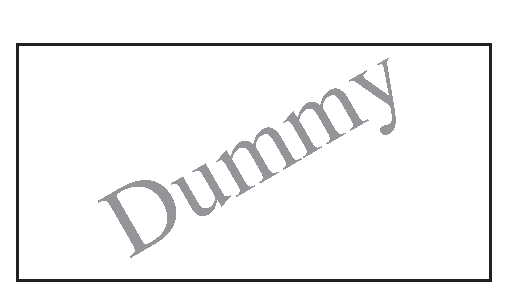
\includegraphics[width=12cm]{dummy.eps}
\end{center}
\caption{You can put EPS files into the document.}
\label{f1}
\end{figure}

\section{Comments}

If you have trouble or find a bug, please e-mail the Online-Journal Subcommittee of JPSJ\@.~\cite{jps}  Your comments on this class file will be welcome.

\begin{thebibliography}{9}

\bibitem{blue} L. Lamport: \textit{\LaTeX: A Document Preparation System} (Addison-Wesley, Reading, 1994) 2nd ed., Translation by H. Abe (Pearson Education, Tokyo, 1999) [in Japanese].

\bibitem{companion} M. Goossens, F. Mettelbach and A. Samarin: \textit{The \LaTeX{} Companion} (Addison-Wesley, Reading, 1994) Translation by ASCCII Corp.\ (ASCII, Tokyo, 1998) p.~257 [in Japanese].

\bibitem{linebyline} A. Diller: \textit{\LaTeX{} Line by Line} (John Wiley \& Sons, Chichester, 1999) 2nd ed., p.~129.

\bibitem{jps} E-mail address is \texttt{jpsj-online@jps.or.jp}

\end{thebibliography}
\end{document}
